% SUSY lectures for 1st year PhDs
\documentclass{beamer}
\usepackage{epstopdf}
\usepackage{pifont}
\usetheme{iclpt}

\newcommand{\mHu}{m_{H_{u}}}
\newcommand{\mHd}{m_{H_{d}}}
\newcommand{\Rbsg}{R(b\rightarrow s\gamma)}
\newcommand{\Rbtn}{R(b\rightarrow \tau\nu)}
\newcommand{\BRbsmumu}{BR(B_{s}\rightarrow\mu^{+}\mu^{-})}
\newcommand{\Ohsq}{\Omega h^{2}}
\newcommand{\Spsi}{\sigma_{p}^{\textrm{SI}}}

\begin{document}

\title{Phenomenology of supersymmetry}
\subtitle{\textcolor{gray}{(and a bit of theory)}}
\author{Sam Rogerson}
\institute{Imperial College London}
\date{\today}

\begin{frame}[plain]
  \titlepage
\end{frame}

\begin{frame}{Outline}
  \tableofcontents [part=1,hideallsubsections,]
  \tableofcontents [part=2,hideallsubsections,] 
  \tableofcontents [part=3,hideallsubsections,] 
  \tableofcontents [part=4,hideallsubsections,] 
  \tableofcontents [part=5,hideallsubsections,] 
\end{frame}


%%%%%%%%%%%%%%%%%%%%%%%%%%%%%%%%%%%%%%%%%%%%%%%%%%%%%%%%%%%%%%%%%%%%%%%%%%%%%%%
% Why we need BSM
%---------------------------------
\part{Why we need BSM physics}
\section{Why we need BSM physics}
\frame{\partpage}
%---------------------------------
\subsection{Standard Model}
\begin{frame}{\insertsubsection}
  Plenty of evidence in favour of the Standard Model:
  \begin{itemize}
    \item Predictions: Existence of W boson,Z boson, charm quark, top quark and the gluon.
    \item Electroweak precision measurements: Mass and width of W and Z bosons.
  \end{itemize}
  It is, as you know, not complete
\end{frame}

\subsection{What it doesn't include}
\begin{frame}{\insertsubsection}
  \begin{itemize}
    \item Neutrino masses (Dirac/Majorana): can add terms, but not a direct
    result \alert{[essential]}
    \item Gravity
    \item Dark Matter (`orthogonal' measurement)
  \end{itemize}
\end{frame}

\subsection{What does it get ``wrong''?}
\begin{frame}{\insertsubsection}
  \begin{itemize}
    \item Anomalous Magnetic Moment of the Muon: $(g-2)_{\mu}$
    \item Natural solution to W-scattering cross-section
    \item Higgs mass \alert{[?]}
  \end{itemize}
  There is also the problem of \textit{naturalness}:
  \begin{itemize}
    \item Why do we need 19 parameters to describe the SM?
    \item Why do we have a hierarchy problem? (Fine tuned cancellations to
    Fermi's constant)
  \end{itemize}
\end{frame}

\subsection{What is the hierarchy problem?}
\begin{frame}{\insertsubsection}
  \begin{itemize}
    \item Suppose SM valid up to GUT scale ($O(10^{15}\textrm{GeV})$) or even
    the Planck scale ($O(10^{19}\textrm{GeV})$)
    \item Weak interaction scale $\sim100\textrm{GeV}$
    \item If the inputs are chosen at these scales, the scalar mass terms in
    the Higgs sector must be chosen with an accuracy of $10^{-34}$ wrt the
    Planck mass.
  \end{itemize}
\end{frame}

\subsection{W-scattering cross-section}
\begin{frame}{\insertsubsection}
  One of the strongest indicators for something Higgs-like/BSM physics:
  \begin{itemize}
    \item Theory: the value explodes at some energy scale
    \item Violates perturbative unitarity
    \item Simplest solution: extra propagator = extra diagram $\rightarrow$
    cancels divergences
    \item This propagator is a scalar $\rightarrow$ Higgs
    \item Good evidence for upper limit on Higgs mass
  \end{itemize}
\end{frame}

\subsection{Divergent Higgs Mass}
\begin{frame}{\insertsubsection}
  \center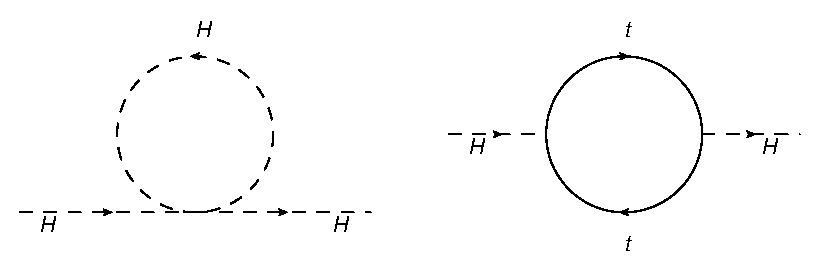
\includegraphics[scale=0.4]{oneloop.eps}\\
  The one loop scalar(left) and fermion(right) corrections to the Higgs mass.
  When calculated we find the following contributions:
  \begin{itemize}
    \item dirac fermion ($-\lambda_{f}\bar{f}f$):
    $\Delta m_{H}^{2}=-\frac{|\lambda_{f}|^2}{8\pi^{2}}\alert{\Lambda_{UV}^{2}}
    +\hdots$ 
    \item $\mathbb{C}$-scalar($-\lambda_{S}|H|^{2}|S|^{2}$): 
    $\Delta m_{H}^{2}= \frac{\lambda_{S}}{16\pi^{2}}\left[\Lambda_{UV}^{2}-2
    \alert{m_{S}^{2}}\ln\left(\Lambda_{UV}/m_{S}\right) \right]$
  \end{itemize}
  Here $\Lambda_{UV}$ is known as the `ultraviolet' cutoff - it regulates the loop
  integral, i.e $M=\int_{0}^{\Lambda_{UV}}\hdots$
\end{frame}

\subsection{Divergent Higgs Mass Part 2}
\begin{frame}{\insertsubsection}
  These corrections imply two important things:
  \begin{enumerate}
    \item A quadratic dependence on $\Lambda_{UV}$
    \item A quadratic dependence on $m_{S}$
  \end{enumerate}
  This means it is both sensitive to the scale of `new-physics', as well as the
  masses of the heaviest particles.  Strangely enough the latter problem arises
  even if we have no direct coupling between the SM Higgs and the unknown
  ``$S$''.
  \vfill\hfill We'll come back to this...
\end{frame}

\subsection{Why it could be SUSY}
\begin{frame}{\insertsubsection}
  \textcolor{gray}{Phenomenologically}
  While we haven't developed the details, yet, the extended particle spectrum
  gives hints at what it \alert{could} provide,
  \begin{itemize}
    \item Corrections to $\Delta(g-2)_{\mu}$
    \item A candidate for dark matter.
    \item Cancellation terms for the Higgs mass
    \item A solution to the Hierarchy problem
  \end{itemize}
\end{frame}


%%%%%%%%%%%%%%%%%%%%%%%%%%%%%%%%%%%%%%%%%%%%%%%%%%%%%%%%%%%%%%%%%%%%%%%%%%%%%%%
% Constructing SUSY
%---------------------------------
\section{Constructing the details of SUSY}
\part{Constructing the details of SUSY}
\frame{\partpage}
%---------------------------------

\subsection{Multiplets}
\begin{frame}{\insertsubsection}
In the standard model we arrange particles into the \alert{irreducible
representations} of the
algebra called multiplets,
  \begin{equation*}
    \binom{e_L}{\nu_{e}},\binom{u_{L}}{d_{L}}
  \end{equation*}
A similar approach is taken for SUSY; we form \alert{supermultiplets}, simply an
arrangement which contains both fermion and boson partner states
\end{frame}

\subsection{Multiplets Continued}
\begin{frame}{\insertsubsection}
  If $\left|\Omega\right>$ and $\left|\Omega^{\prime}\right>$ are both members of
  the same supermultiplet, then they are linear combinations of each other (with
  the SUSY operator $\hat{O}$ and $\hat{O}^{\dagger}$).
  \\ When constructing these multiplets we must ensure:
  \begin{equation*}
    n_{B}=n_{F}
  \end{equation*}
  where $n_{B}$ and $n_{F}$ are the bosonic and fermionic degrees of freedom
  respectively (this can be shown).
\\
  \alert{The simplest arrangement: single weyl fermion (2 spin states, $n_{F}=2$) and
  then 2 real scalars ($n_{B}=1$ each)}
\end{frame}

\subsection{More Multiplets}
\begin{frame}{\insertsubsection}
\textcolor{gray}{Note:
$2\times\mathbb{R}\textrm{-scalar}\equiv1\times\mathbb{C}\textrm{-scalar}$}\\
  The next simplest arrangement is a spin-1 vector boson ($n_{B}=2$), with a
  massless Weyl fermion as its superpartner.
  \\
  These two arrangements have names:
  \begin{itemize}
    \item spin-$1/2$ Weyl Fermion + $\mathbb{C}$-scalar: \alert{Chiral
    supermultiplet}
    \item spin-1 Vector boson + massless Weyl fermion: \alert{Gauge
    supermultiplet}
  \end{itemize}
\end{frame}

  
\subsection{Breaking SUSY}
\begin{frame}{\insertsubsection}
  If SUSY were an exact symmetry of the Lagrangian, then we would have,
  \begin{equation*}
    M_{\textrm{SM}}=M_{\textrm{SUSY}}
  \end{equation*}
  for all particles. If this were true, SUSY would be evident in experiments
  already.  We therefore expect SUSY to be broken to some degree, i.e. the mass
  scale of the particles is not completely restricted.
\alert{There is a much better reason than this...}
\end{frame}

\subsection{What is a gauge anomaly}
\begin{frame}{\insertsubsection}
  \begin{definition}
  A gauge anomaly is \alert{any} effect that breaks the gauge symmetry of the system, in our case the
  quantum field theory.
  \end{definition}
\end{frame}

\subsection{The Higgs Sector}
\begin{frame}{\insertsubsection}
  Naively one would expect the following:
  \begin{equation*}
    \textrm{Higgs } H \leftrightarrow \tilde{H}\textrm{ Higgsino} 
  \end{equation*}
  There is a \textcolor{gray}{(two)} problem\textcolor{gray}{(s)} with this,
  \begin{itemize}
    \item Introduction of a gauge anomaly, namely Higgsino ($S=\pm1/2$) has hypercharge
    $\textrm{Y}=\frac{1}{2}$, so we no longer have $\sum\textrm{Y}=0$ (our
    $U(1)$ gauge symmetry has been broken)
  \end{itemize}
\end{frame}

\subsection{The Higgs Sector Continued}
\begin{frame}{\insertsubsection}
  Can remedy this gauge anomaly by introducing a second higgs doublet, labelling
  the two (unsuggestively) $H_{u}$ and $H_{d}$.
  \begin{itemize}
    \item Opposite hypercharge (fixes the anomaly)
    \item $H_{u}$ now couples to up-type fermions ($u,c,t,\ell$)
    \item $H_{d}$ couples to down-type fermions ($d,s,b,\nu_{\ell}$)
  \end{itemize}
\end{frame}

\subsection{Supersymmetry is...}
\begin{frame}{\insertsubsection}
A symmetry that generates a second set of particles matching those in the SM
but with masses at a higher scale.
\begin{itemize}
  \item Each boson(fermion) has a corresponding (fermion)boson superpartner
  \item A second Higgs doublet is included, resulting in 5 physical Higgs bosons
\end{itemize}

\end{frame}

%%%%%%%%%%%%%%%%%%%%%%%%%%%%%%%%%%%%%%%%%%%%%%%%%%%%%%%%%%%%%%%%%%%%%%%%%%%%%%%
% Models of supersymmetry
%---------------------------------
\section{Models of supersymmetry}
\part{Models of supersymmetry}
\frame{\partpage}
%---------------------------------
\subsection{Minimal Supersymmetric Standard Model}
\begin{frame}{\insertsubsection}
  So far we have constructed what is known as the Minimal Supersymmetric
  Standard Model (MSSM)   
  \begin{itemize}
    \item super-partners for each SM particle
    \item softly-broken (mass differences, but no quadratic divergences)
  \end{itemize}
  This was motivated by the SM seeming ``unnatural'',
  \begin{itemize}
    \item  Number of parameters (19)
    \item  Energy scale ($M_{pl}$ vs. $M_{W}$)
  \end{itemize}
\end{frame}

\subsection{Not so natural...}
\begin{frame}{\insertsubsection}
  Unfortunately we have only really solved one of these problems,
  \begin{tabular}{l l }
    \checkmark & Energy scale \textcolor{gray}{[almost]}\\
    \ding{55} & Parameters \\
  \end{tabular}
  \\ To fully specify all the masses and couplings in the MSSM we need 108 free
  parameters.
  \\ \alert{Solution:} Choose some `natural` boundary condition to alleviate
  this problem.
\end{frame}

\subsection{Constrained MSSM}
\begin{frame}{\insertsubsection}
  Motivating unification,
  \rotatebox{90}{\textcolor{gray}{Standard model}}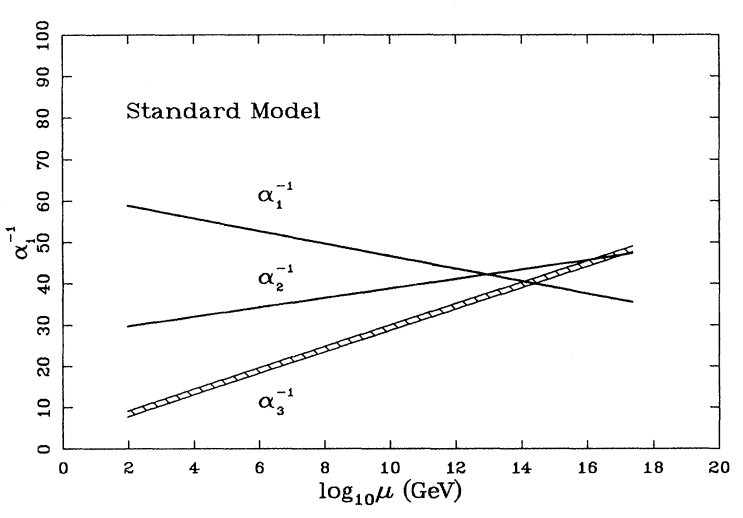
\includegraphics[height=3.5cm]{couple_sm.png}
  \rotatebox{90}{\textcolor{gray}{MSSM}}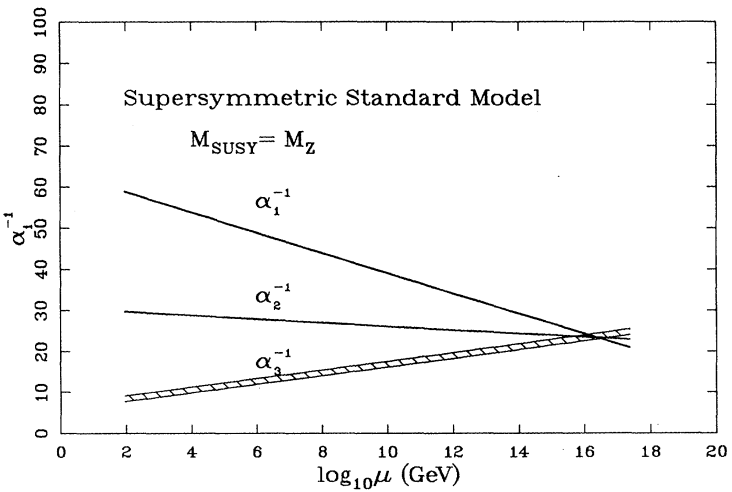
\includegraphics[height=3.5cm]{couple_susy.png}
\end{frame}

\subsection{CMSSM: A gut scale condition}
\begin{frame}{\insertsubsection}
We now impose another GUT scale constraint
\begin{itemize}
    \item Scalar masses unify = $m_{0}$
    \item Gaugino masses unify = $m_{1/2}$
    \item Trilinear couplings unify = $A_{0}$
\end{itemize}
This \emph{almost} gives us a complete description of the physics, just need to
describe the Higgs sector,
\begin{itemize}
    \item Two higgs fields - $\phi_{H_{u}}/\phi_{H_{d}} = \tan\beta$
\end{itemize}

\end{frame}

\subsection{cMSSM: Dragging it out...}
\begin{frame}{\insertsubsection}
While phenomenologically \emph{not} the most interesting:
\begin{itemize}
    \item Simple unification collapses parameter space
    \item \emph{Forces ration between the gauge couplings}
\end{itemize}
This last point is important for the phenomenology.  Consider the following
decay:
\begin{equation*}
    \tilde{g}\rightarrow\tilde{q}\rightarrow\tilde{\chi}^{0}_{1}
\end{equation*}
If the couplings are fixed, then the mass ratios are also fixed
\begin{equation*}
    6:4:1
\end{equation*}
\end{frame}

\subsection{NUHM}
\begin{frame}{\insertsubsection}
While there is \textit{some} motivation for models like the cMSSM, the
phenomenology is not wide ranging  NUHM models are an attempt to remedy that via
the introduction of a new degree(s) of freedom,
\begin{itemize}
    \item \emph{NUHM1} $\mHu = \mHd \neq m_{0}$
    \item \emph{NUHM2} $\mHu \neq \mHd \neq m_{0}$
\end{itemize}
\end{frame}

\subsection{Some common confusion}
\begin{frame}{\insertsubsection}
\emph{SUSY adds a new set of partner particles to the SM}
\begin{itemize} 
    \item Commonly talk about \emph{neutralinos} and \emph{charginos}
    \item No obvious SM partner for these particles
    \item Actually combinations of the photino ($\tilde{\gamma}$),
    bino ($\tilde{B}$), wino ($\tilde{W}$) and higgsino ($\tilde{H}$) fields.
\end{itemize}
\end{frame}

%%%%%%%%%%%%%%%%%%%%%%%%%%%%%%%%%%%%%%%%%%%%%%%%%%%%%%%%%%%%%%%%%%%%%%%%%%%%%%%
% What now?
%---------------------------------
\section{What now?}
\part{What now?}
\frame{\partpage}
%---------------------------------
\subsection{Understaning the models}
\begin{frame}{\insertsubsection}
\begin{itemize}
    \item Nice to have models that are `theoretically motivated'
    \item Do they match with Experiment?
\end{itemize}
There are `indirect' tests of supersymmetry, can also act as constraints.
\end{frame}

\subsection{Constraints}
\begin{frame}{\insertsubsection}
There are, literally, thousands of measurements in physics.  Can choose a
handful that \emph{should} be sensitive to supersymmetric effects
\begin{columns}[c]
    \column{0.5\textwidth}
    \begin{itemize}
        \item  Flavour physics
        \begin{itemize} 
            \item $\Rbsg$
            \item $\BRbsmumu$
            \item $\Rbtn$
        \end{itemize}
        \item Higgs searches (LEP)
    \end{itemize}
    \column{0.5\textwidth}
    \begin{itemize}
        \item Cosmological
        \begin{itemize}
            \item $\Ohsq$
            \item $\Spsi$
        \end{itemize}
        \item Direct searches (TeVatron, \emph{CMS}, ATLAS)
    \end{itemize}
\end{columns}
\end{frame}

\subsection{Attacking SUSY parameter space}
\begin{frame}{\insertsubsection}
While there aren't any true limits on SUSY-parameters,
\begin{itemize}
    \item For each set of inputs \{ $m_{0}$, $m_{1/2}$, $A_{0}$, $\tan\beta$,
    $\hdots$ \} there is a uniquely defined spectrum of particles
    \item In fact for all \{$\hdots$\} all other values are defined (as you'd expect)
\end{itemize}
\end{frame}

\subsection{Turning this into constraints}
\begin{frame}{\insertsubsection}
We know the phenomenology (through the masses and couplings) is well defined for
any set of input parameters to any give model
\begin{itemize}
    \item Calculate spectrum and couplings
    \item Calculate SUSY contribution to expectation value of various
    observables
    \item Compare to current experimental values and accuracy
\end{itemize}

In this way we can construct a method for determining the goodness-of-fit of any
single point in any given model (so long as we can perform the first two steps).
\end{frame}

\subsection{Whole space approach}
\begin{frame}{\insertsubsection}
For some models it is possible to do this for a wide enough selection of points
that we end up with well defined regions of best fit\\
This allows us to determine the most `important' input parameters, and if they
exist the observables that drive the sort of phenomenology we might expect to
see
\end{frame}

\subsection{What do we get?}
\begin{frame}{\insertsubsection}
What might you execpt?
\begin{itemize}
    \item Low/High masses?
    \item Low/High probability of fit?
\end{itemize}
\end{frame}

\begin{frame}{\insertsubsection}
\begin{columns}[l]
    \column{0.5\textwidth}
    CMSSM\\
    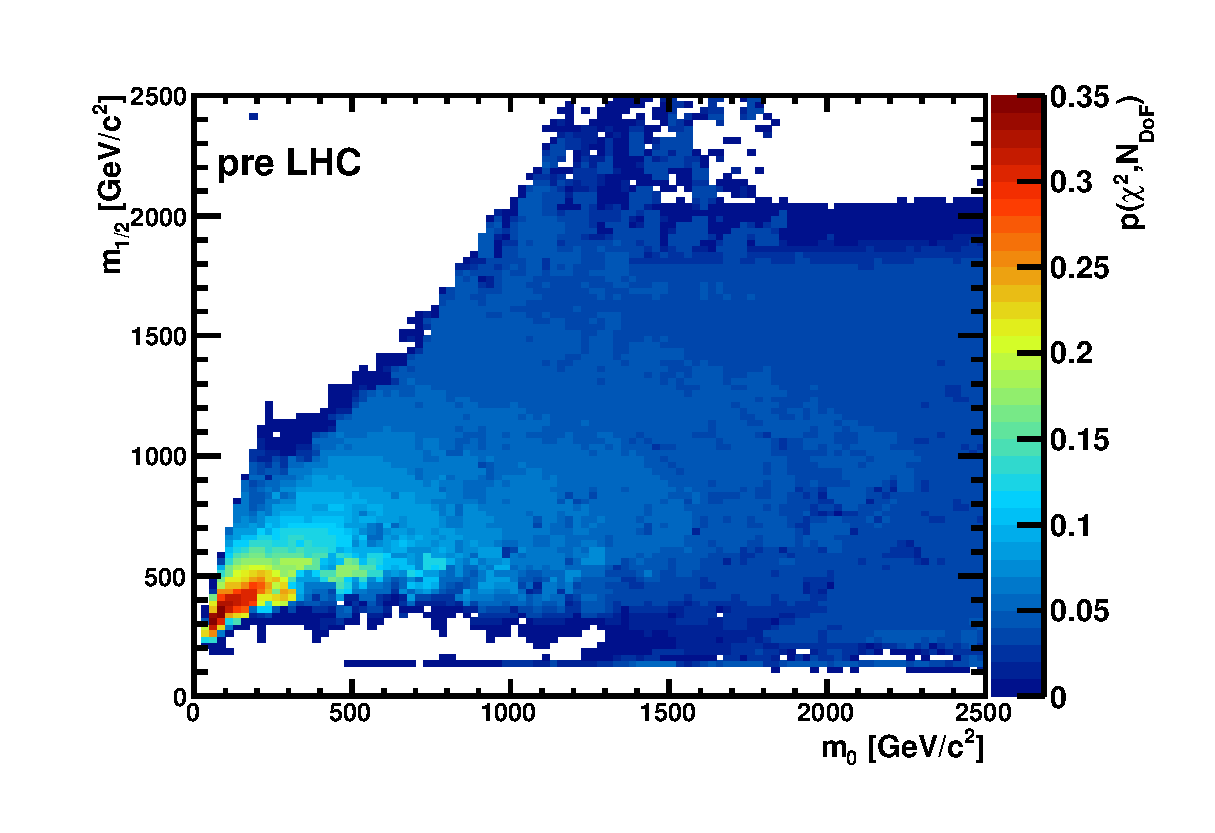
\includegraphics[height=4.2cm]{m0m12_cmssm_px_pre.eps}
    \column{0.5\textwidth}
    NUHM1\\
    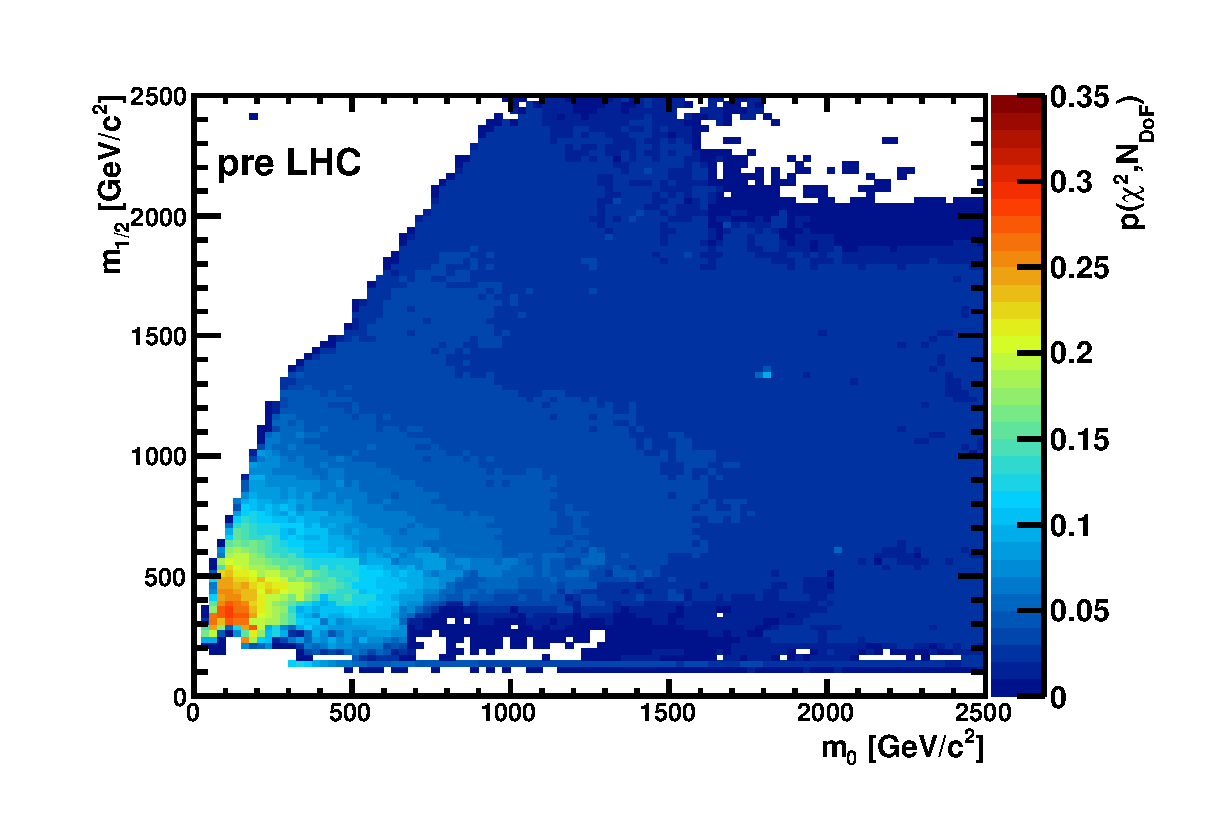
\includegraphics[height=4.2cm]{m0m12_nuhm1_px_pre.eps}\\
\end{columns}
\end{frame}

\begin{frame}{\insertsubsection}
\begin{columns}[l]
    \column{0.5\textwidth}
    CMSSM\\
    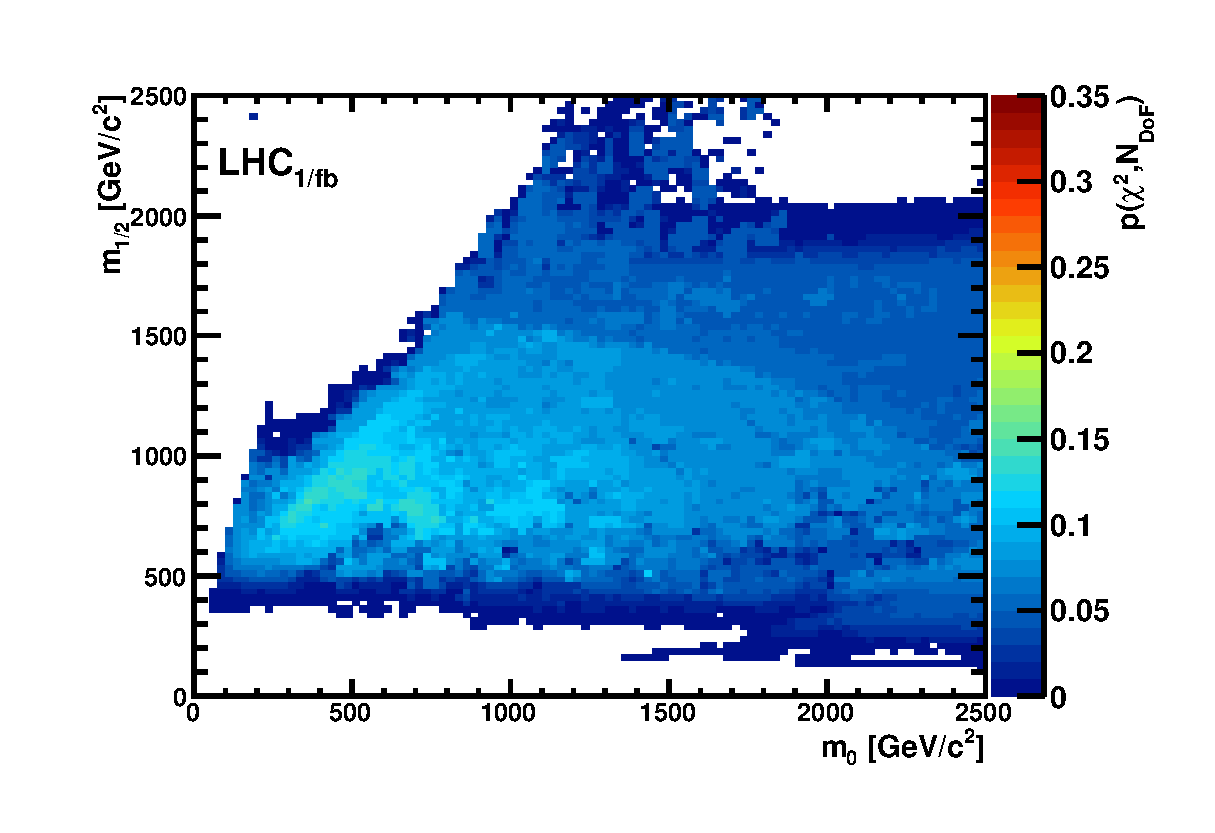
\includegraphics[height=4.2cm]{m0m12_cmssm_px_eps_comp.eps}
    \column{0.5\textwidth}
    NUHM1\\
    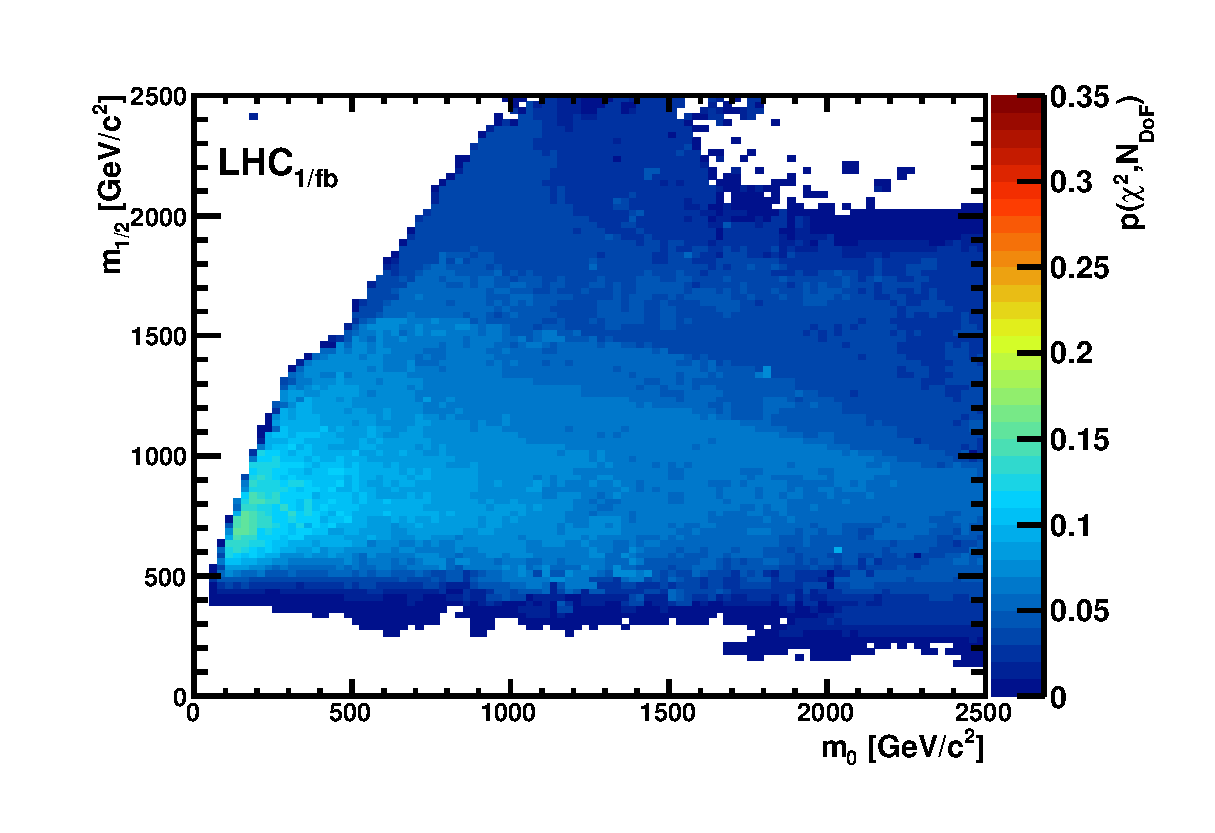
\includegraphics[height=4.2cm]{m0m12_nuhm1_px_eps_comp.eps}\\
\end{columns}
\end{frame}

\subsection{What else can we determine}
\begin{frame}{\insertsubsection}
Parameter space plots are useful for discussions of the model directly, but we
can determine the preferred region for phenomenologically interesting values,
such as (s)particle masses
\end{frame}

\subsection{Higgs Mass}
\begin{frame}{\insertsubsection}
\begin{columns}[l]
    \column{0.5\textwidth}
    CMSSM\\
    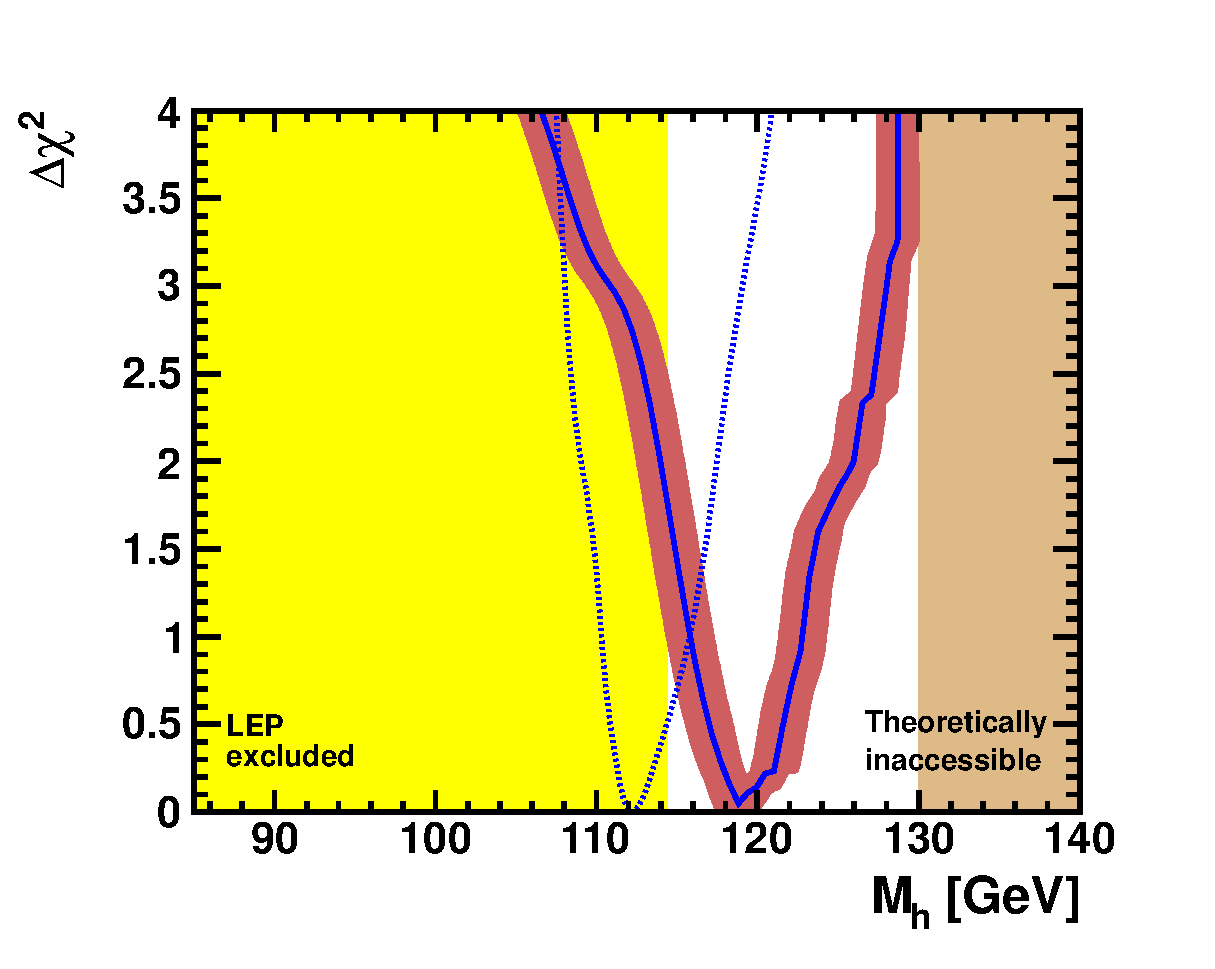
\includegraphics[height=4.2cm]{mh_cmssm.eps}
    \column{0.5\textwidth}
    NUHM1\\
    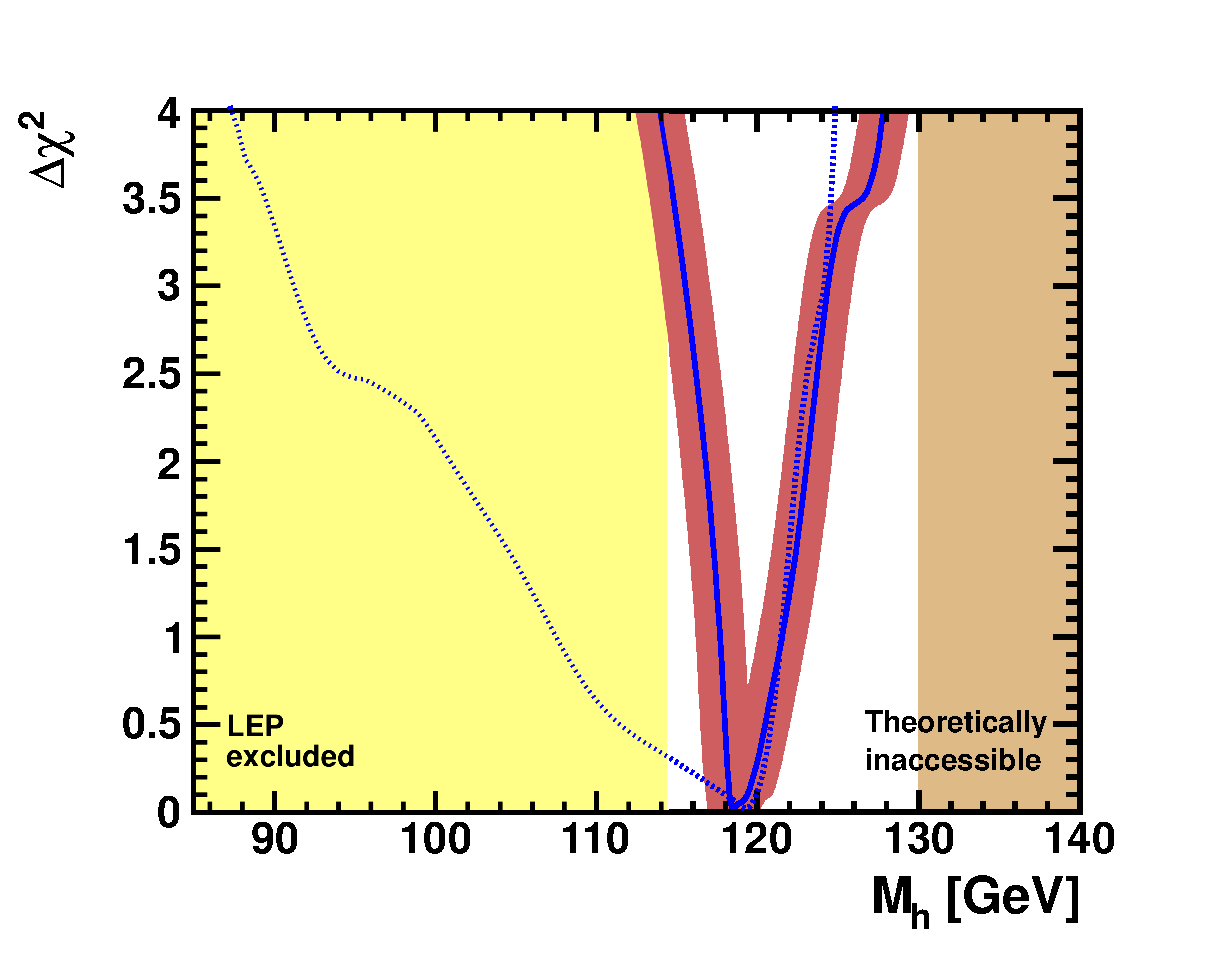
\includegraphics[height=4.2cm]{mh_nuhm1.eps}\\
\end{columns}
\end{frame}

%%%%%%%%%%%%%%%%%%%%%%%%%%%%%%%%%%%%%%%%%%%%%%%%%%%%%%%%%%%%%%%%%%%%%%%%%%%%%%%
% Summary
%---------------------------------
\section{Summary}
\part{Summary}
%---------------------------------
\subsection{Summary}
\begin{frame}{\insertsubsection}
\begin{itemize}
    \item SUSY seems to be a "cure-all" for problems with the SM
    \item Simple models can be constructed (CMSSM, NUHM1)
    \item These can be tested against experiment
    \item We still haven't seen any signals of SUSY
    \item Seems likely that more complicated / different models may yet be
    necessary
\end{itemize}
\end{frame}

\end{document}


